%%%%%%%%%%%%%%%%%%%%%%%%%%%%%%%%%%%%%%%%%%%%%%%%%%%%%%%%%%%%%%%%%%%%%%%%
%
%   Folien: SMT Workshop
%           SMTInterpol
%   Juli 2021
%
%%%%%%%%%%%%%%%%%%%%%%%%%%%%%%%%%%%%%%%%%%%%%%%%%%%%%%%%%%%%%%%%%%%%%%%%

\documentclass[table,aspectratio=169]{beamer}
\usepackage{xcolor}

\usepackage{tikz}
\usetikzlibrary{fit,shapes.callouts,shapes.geometric,shapes.symbols}
\usetikzlibrary{positioning,calc}

\usetheme{Madrid}
\usecolortheme{freiburg}
\useoutertheme{unifr}
\setbeamertemplate{navigation symbols}{}
\setbeamertemplate{itemize/enumerate subbody begin}{\normalsize}

\let\checkmark\relax
\usepackage{dingbat}

%%% Titel, Autor und Datum des Vortrags:
\pgfdeclareimage[height=1cm]{unifr}{unifr-neu}

%% Institut
\institute[Uni Freiburg]{University of Freiburg\hspace{1cm}\pgfuseimage{unifr}}


\begin{document}

\begin{frame}[plain,fragile]
  \frametitle{SMTInterpol and SMTInterpol-remus}
  \framesubtitle{J\"{u}rgen Christ, Leonard Fichtner, Jochen Hoenicke, Moritz Mohr, Tanja Schindler}
  \pgfdeclarelayer{back}
  \pgfsetlayers{back,main}
  
  \vspace{1ex}
  \begin{columns}[t]
  \begin{column}{.5\textwidth}
  Interpolating SMT solver
    \begin{itemize}
    \item based on CDCL(T)
      
    \item for Arrays, Uninterpreted Functions, Linear Integer and Real Arithmetic
    \begin{itemize}
      \item plus \texttt{div} and \texttt{mod} with constants,
    \end{itemize}
    and \alert{DataTypes}
    
    \item supports quantifiers
    
    \item produces models, proofs, and unsat cores
    
    \item computes sequence and tree interpolants
    \end{itemize}
  \end{column}
  
  \hfill\textcolor{ALUblue}{\vrule width 1pt }\hfill{}
  
  \begin{column}{.5\textwidth}
    SMTInterpol at SMT-COMP 2021
    \begin{itemize}
    \item with \alert{proof check mode enabled}
    
    \item experimentally participated in\\
    some \alert{Nonlinear Arithmetic} divisions
      
    \item variant SMTInterpol-remus with\\
    \alert{unsat core enumeration}
    \end{itemize}
  \end{column}
  \end{columns}
  \begin{center}
    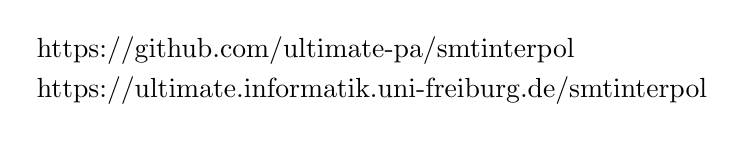
\begin{tikzpicture}
      \node[anchor=west] (url) at (-5,-.5)
      {\url{https://github.com/ultimate-pa/smtinterpol}};
      \node[anchor=west] (url) at (-5,-1)
      {\url{https://ultimate.informatik.uni-freiburg.de/smtinterpol}};
    \end{tikzpicture}
  \end{center}
\end{frame}
\end{document}
